\chapter{From Summit to Success: Thresholds of Load and the Discipline of Descent}

This interview excerpt begins with a practical question about books, but it quickly becomes a compact theory of overload. The speaker starts from early success and hypergrowth, passes through a period of stress without diagnosis, and then finds in \emph{Into Thin Air} an analogy strong enough to explain why capable people begin to fail when the scale of the company outruns the scale of the role. The mathematics here is necessarily cautious and editorial, but the lecture does support a clean threshold picture: load accumulates, thresholds differ, collapse is nonlinear, and leadership means reducing load before failure is mistaken for weakness.

\section{Opening Context and the Book Question}

The opening is clipped and immediate. The speaker does not begin with a neutral recommendation list; he begins with the fact that he had a high-tech company and achieved success very young. That matters, because the later answer about books is not being offered as literary taste. It is being offered as hard-won operating judgment.

The interviewer then asks for three books that any entrepreneur should read. The answer narrows almost immediately to one book, and that narrowing gives the section its shape. We are not about to receive a balanced bibliography. We are about to receive a single case in which a book became an interpretive instrument.

\section{Hypergrowth Without a Diagnosis}

The next move is to slow the story down. At the time, the business was growing very fast, the days were intensely stressful, and yet the speaker could not identify the underlying defect in the system. This is the essential setup: the business is not failing because the speaker lacks effort, and it is not even obviously failing because of one visible decision. The difficulty is diagnostic.

That is why the reading moment matters. He comes home after punishing days and reads partly in order to sleep, and it is in that setting that \emph{Into Thin Air} enters the argument. The book is not decoration. It becomes a way to name a problem that had previously been experienced only as pressure.

\section{Into Thin Air and the Threshold Model}

The decisive phrase is that ``it clicked.'' From that point on, the lecture proceeds by analogy. In the mountain story, people go upward in altitude, oxygen becomes scarce, and even simple tasks begin to feel surprisingly difficult. Crucially, people are built differently, so the relevant limit is not universal. One person continues; another reaches a threshold and begins to fail.

\begin{definition}
Let \(L_i(t)\) denote the effective role load carried by person \(i\) at time \(t\), and let \(C_i\) denote that person's current operating capacity. We shall call person \(i\) overloaded when
\begin{equation}
L_i(t) > C_i.
\end{equation}
\end{definition}

\begin{remark}
This notation is a cautious formalization of the speaker's analogy, not a quoted equation from the interview. The lecture itself is verbal, but it clearly distinguishes between a manageable regime and a regime in which performance degrades after a personal threshold is crossed.
\end{remark}

The mountain picture may be written in the same spirit. If \(h\) denotes altitude and \(h_i^\ast\) the threshold altitude for person \(i\), then the lecture's logic is

\begin{equation}
h > h_i^\ast \Longrightarrow \text{even simple tasks become difficult for person } i.
\end{equation}

This is the first essential move. The difficulty is not merely that work exists. The difficulty is that work crosses a threshold. The speaker also notes that without intervention the situation becomes dangerous, and the only solution in the mountain story is to go down.

\begin{figure}
\centering
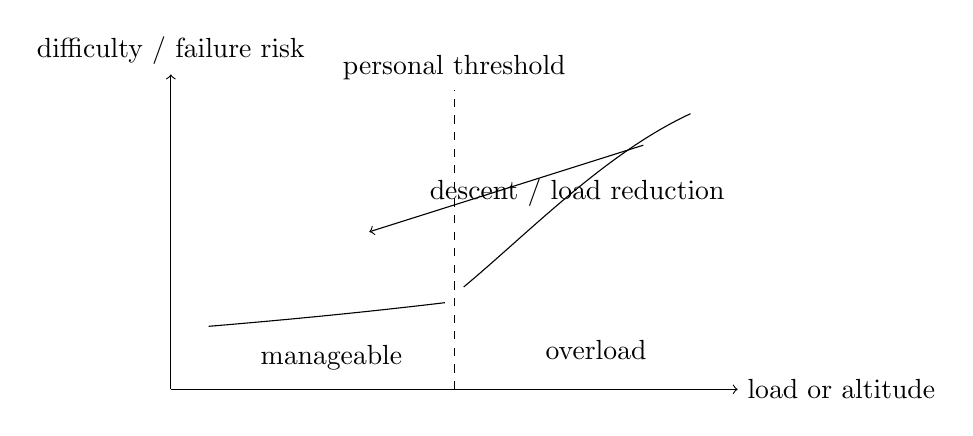
\begin{tikzpicture}[x=1.2cm,y=1cm]
\draw[->] (0,0) -- (6,0) node[right]{load or altitude};
\draw[->] (0,0) -- (0,4) node[above]{difficulty / failure risk};
\draw[dashed] (3,0) -- (3,3.8);
\draw (0.4,0.8) .. controls (1.4,0.9) and (2.2,1.0) .. (2.9,1.1);
\draw (3.1,1.3) .. controls (3.8,2.0) and (4.6,3.0) .. (5.5,3.5);
\node at (1.7,0.4){manageable};
\node at (4.5,0.5){overload};
\node[above] at (3,3.8){personal threshold};
\draw[->] (5.0,3.1) -- (2.1,2.0);
\node at (4.3,2.5){descent / load reduction};
\end{tikzpicture}
\caption{Editorial schematic of the threshold logic implicit in the lecture: performance may look stable up to a personal limit, and intervention consists in reducing load rather than treating the person as morally defective.}
\end{figure}

\subsection{Question \& Answer}

\paragraph{Question.} Why do capable employees begin to fail when the company scales?

\paragraph{Answer.} The lecture's answer is that the role has changed faster than the person. At one stage we have
\begin{equation}
L_i(t) \le C_i,
\end{equation}
and the same individual looks effective. Later, with the company larger and the role heavier, we have
\begin{equation}
L_i(t) > C_i,
\end{equation}
and the same individual now looks as though he is failing. The conceptual gain is large: what appears to be personal decline is reinterpreted as a mismatch between load and capacity.

This is precisely why the mountain analogy comes before the organizational diagnosis. The lecture first teaches us how thresholds work in a vivid external setting, and only then returns to the company to say: this is what was happening here.

\section{A Worked Example of Role Expansion}

The speaker then makes the picture concrete. Someone who had been managing \(4\), \(6\), or \(10\) people may, six months or a year later, be managing \(20\) or \(30\). Those numbers matter because they convert a general feeling of stress into a discrete change of scale.

Let \(n_i(t)\) denote the number of people managed by person \(i\) at time \(t\). The transcript supports examples of the form
\begin{align}
n_i(t_0) &= 6,  & n_i(t_1) &= 20,  & \Delta n_i &= 14, \\
n_i(t_0) &= 10, & n_i(t_1) &= 30,  & \Delta n_i &= 20.
\end{align}

As a deliberately simple proxy, let us suppose that effective load grows in proportion to span of control:
\begin{equation}
L_i(t) = \alpha\, n_i(t),
\end{equation}
where \(\alpha > 0\) is not measured but merely records that more reports typically mean more coordination, judgment, interruption, and responsibility.

Then the change in load is
\begin{equation}
\Delta L_i = L_i(t_1)-L_i(t_0)=\alpha\bigl(n_i(t_1)-n_i(t_0)\bigr)=\alpha\,\Delta n_i.
\end{equation}

Now suppose, for one employee, that
\begin{equation}
6\alpha \le C_i < 20\alpha.
\end{equation}
At the first time the role is manageable; at the second time the same person has crossed the threshold. Nothing in this toy calculation says the person became weaker. The lecture's point is almost the opposite: the organization changed the problem faster than the person could adapt to it.

\section{Juggling and Nonlinear Failure}

The speaker then switches analogies again, but not to change the idea. He uses juggling to sharpen it. If one can juggle three balls, then perhaps one can take a fourth, then a fifth, then a sixth. For a while the system appears stable. That appearance is deceptive.

Let \(b\) denote the number of balls being juggled and \(b_i^\ast\) the maximum stable load for person \(i\). The lecture's discrete threshold may then be written as
\begin{equation}
b > b_i^\ast \Longrightarrow \text{the balls are dropped.}
\end{equation}

\begin{proposition}
The lecture treats overload as threshold-like rather than smoothly proportional.
\end{proposition}

\begin{proof}
In the juggling example, the speaker does not describe a steady fractional decline after each additional ball. He describes continued competence as more load is added and then, after a personal limit is exceeded, a visible collapse in performance. The image is therefore one of nonlinear breakdown, not of gradual moral deterioration.
\end{proof}

This is one of the most useful moments in the excerpt. Juggling strips the idea of drama and leaves the structure bare. More load is not always immediately catastrophic. That is why organizations can overburden people without noticing it. But once the threshold is crossed, the resulting failure can look sudden and total.

\section{Managerial Descent and the Ethics of Intervention}

The final movement of the excerpt is managerial. Once the speaker realizes that people are not necessarily failing from laziness or lack of will, responsibility shifts upward. The leader's task is to stop adding load blindly and, in some cases, to take people ``down the mountain.'' The transcript is rough in this passage, but the direction is clear.

In the language of our notation, the intervention is not an exhortation to try harder. It is a reduction of load:
\begin{equation}
L_i(t+1) = L_i(t) - \Delta_i,
\qquad
\Delta_i > L_i(t)-C_i.
\end{equation}
If this inequality holds, then after intervention we have \(L_i(t+1) < C_i\), and the role becomes tractable again.

There are two concrete forms of this intervention in the logic of the lecture:
\begin{itemize}
\item stop handing the person more balls;
\item in some cases, move the person to a lower-load position, which is the organizational analogue of descending the mountain.
\end{itemize}

This is the moral center of the excerpt. A company that is scaling rapidly will be tempted to interpret every shortfall as a defect in the individual. The lecture resists that temptation. It asks us first to inspect the structure of the load.

\section{Summary}

The excerpt begins as a recommendation about books and ends as a compact theory of managerial judgment. The book matters because it gives the speaker a threshold model: as altitude rises, oxygen runs thin; as load rises, the same person may cross from competence into overload. The decisive insight is that hypergrowth changes jobs faster than it changes people.

The mountain analogy gives the lecture its shape, the direct-report numbers give it operational force, and the juggling image gives it mathematical clarity. Load may accumulate quietly, but failure appears sharply once a personal limit is crossed. The practical conclusion follows at once: leadership is not only the assignment of responsibility; it is the discipline of descent, the willingness to reduce load before human strain is mistaken for personal collapse.